\documentclass[a4paper,11pt,fleqn]{report}

\usepackage{acronym}
\usepackage{amsmath,amssymb,amsfonts}
\usepackage{booktabs}
\usepackage[dvipsnames]{xcolor}
\usepackage[margin=28mm]{geometry}
\usepackage{graphicx}
%	\graphicspath{
%		{.../Graphics/}
%	}
\graphicspath{{graphics/}}
\usepackage{hyperref}
	\hypersetup{
		colorlinks=true,
		linkcolor=blue,
		filecolor=blue,
		urlcolor=blue,
		citecolor=blue
	}
\usepackage[sort&compress]{natbib}
	\bibliographystyle{apalike}
%\usepackage[mark]{gitinfo2}
%\renewcommand{\gitMark}{Branch:\,\gitBranch\,@\,\gitAbbrevHash{}; Author:\,\gitAuthorName; Date:\,\gitAuthorIsoDate~\textbullet{}}
\usepackage{url}

\begin{document}
%===============================================================
% Frontmatter and title page to be added manually at the end
%===============================================================
\thispagestyle{empty}
\begin{center}
{\huge \textit{`e-casa'} - Eco-friendly Household Waste System\\Part II}
\vspace{20mm} \\
{\Large Group 6}
\vfill

A project report in partial fulfilment of the requirements for the subject\\
\vspace{10mm}
{\Large \textsc{Systems Engineering (BSS 410)}} \\
\vfill
%
in the \\
\vspace{20mm}
%
{\Large \textsc{Faculty of Engineering, Built Environment, and \\ 
Information Technology}}\\
%
\vspace{10mm}
{\Large\textsc{University of Pretoria}} \\
%
\vfill
%
\today
\end{center}

\textit{`e-casa'} - Eco-friendly Household Waste System
\pagenumbering{roman}

\chapter*{Executive Summary}
The aim of this project is to create a household waste system System of that will not only reduce the waste produced by a generic household but do so by increasing value to the user. The final deliverable for this project will be a report that details the needs analysis, conceptual design, feasibility and risk assessment of the designed system. The coneptual design will be done with the use of \textit{Core 9} to capture all identified needs accurately and produce system design documentation.

\tableofcontents
\listoffigures\addcontentsline{toc}{chapter}{List of Figures}
\listoftables\addcontentsline{toc}{chapter}{List of Tables}

\chapter*{Acronyms}
\addcontentsline{toc}{chapter}{Acronyms}
\begin{acronym}[ABCDEF]
\acro{e-casa}{Eco-friendly Household Waste System}
\acro{FBD}{Functional Block Diagram}
\acro{SD}{System Dynamics}
\end{acronym}

\chapter{Introduction and Background}
\pagenumbering{arabic}
\setcounter{page}{1}
\acresetall

\section{Problem Background} \label{sec: Problem Background}
Households consume a variety of products and create different wastes. Products may take the form of food items, municipal water, electricity and other consumables which are either used up or discarded after use. Products discarded after use, such as excess food, food and beverage packaging and water exit the household as forms of waste.  Food clippings from preparing dinner or paper-based packaging is often discarded into dustbins alongside plastic and other waste types to be collected and transported to a dump site. Water used at bathroom sinks or showers is sent directly to the the municipal water system after use to be disposed of. Each type of waste generated by a typical residential household requires proceeding systems that will either store, repurpose or discard the waste.
  
Recent trends have made the consumer market ecologically aware of their own waste generation and many systems have been created to reduce the total waste output of a household. Such products include grey water systems, recycling bins and compost containers. There is a growing need for these means to be adpoted but presently no solution on the market that integrates all means into one comprehensive system for homeowners.
  
Because these systems operate independently, the outputs of one system are often not used as inputs to another. Integrating these systems to operate together could provide more value to the user and further reduce household waste. For example: using food clippings (to create a compost heap) and grey water to grow vegetables in one's garden instead of disposing food clippings in a general waste bin and discarding water to the municipal water system directly after its first use. This eliminates the need for compost to be purchased from a store and reduces water consumption.

\section{Project Objective} \label{sec: Project Objective}
The objective of this project is therefore to investigate the possibility of integrating these different systems as one. The intention is to determine whether the potential cost and resource use savings to be earned from such an integrated system outweigh the financial cost and initial inconvenience to install.

\chapter{Concept Development Stage}
\section{Needs Analysis Phase} \label{sec: Needs Analysis Phase}
\subsection{Operational Need Analysis} \label{Ssec: Operational Need}
\ac{e-casa} is a sustainable household waste management system intended to fulfuill the increasingly prevalent need for sustainable living. The need for individuals and households to consume and dispose of resources in a more sustainable manner is becoming ever more pertinent because of increasing strain on the world's most essential natural resources such as water and fossil fuels. The need is driven by the requirement for individuals (and society as a whole) to reduce their negative impact on the environment by re-use, recycling and minimising resource use as these natural resources become more scarce. Successfully meeting this need will not only improve living conditions for societies but importantly alleviate pressure on governments and municipalities who have to manage and distribute these water and electricity resources to the public.
Although regulation does not yet fully drive this need, government encourages and sometimes imposes restrictions to encourage responsible water and electricity use. This is important to develop a sustainable mindset and awareness of waste generation. Because regulation is still limited on the use of these resources, the onus lies with society and individuals who are aware of and want to mitigate their negative impact on the environment.

\ac{e-casa} is aimed at fulfilling the operational need of sustainable living for households by providing a system that makes it possible to manage and dispose of waste responsibly while simultaneously minimising water consumption. \ac{e-casa} is also expected to provide long-term financial benefits to the user in the form of reduced water consumption costs and grocery bills (with some homegrown foods). Furthermore, there is the expected intangible benefit of the system - knowing one's adverse impact on the environment is mitigated.

Due to a lack of solutions currently on the market, there is an opportunity to enter a gap in the market with \ac{e-casa}. However, this gap is anticipated to be small in size as this product will mainly be aimed at high income individuals aware of (and wanting to reduce) their impact on the environment. There is also an opportunity to market this system as a product to middle class individuals who have sufficient capital to purchase such a system now in order to reap the aforementioned financial savings down the line. However, this extension will likely only be possible if the initial cost of the system is not too high for these individuals and the financial savings are substantial enough to persuade this group.\\


\subsection{Operational Objectives}
The overarching objective that \ac{e-casa} is intended to fulfil is to provide sustainable household waste management. This objective is deconstructed into three primary objectives, namely: \textit{Provide Waste Sortation and Storage}, \textit{Reduce Water Consumption} and \textit{Provide long-term cost savings}. Figure~\ref{fig: ecasaOT} shows the operational objectives of the \ac{e-casa} system.\\

\textcolor{red}{Figure~\ref{fig: ecasaOT} is a work in progress of our objective tree thus far.}

\begin{figure}[h!]
\begin{center}
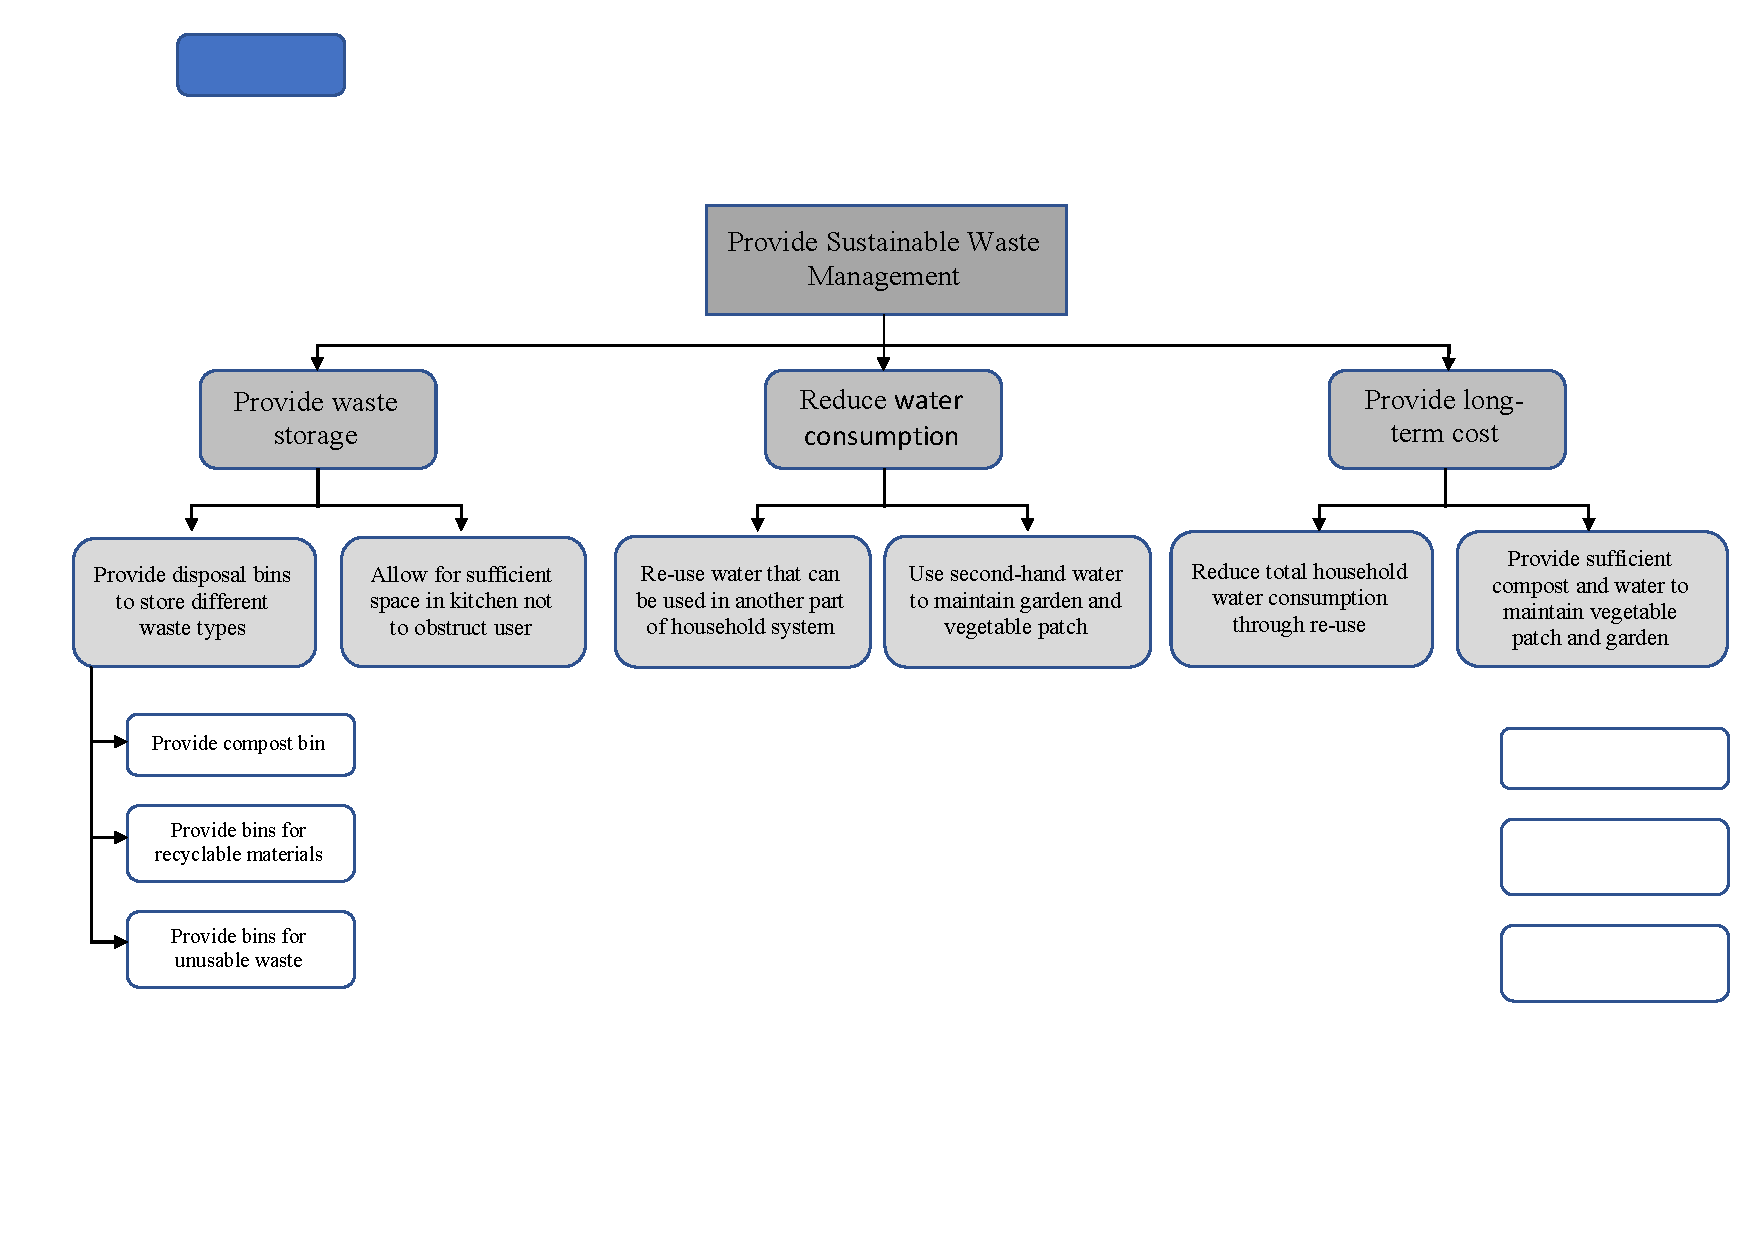
\includegraphics[scale = 0.55]{Objective_Tree_ecasa.pdf}
\caption{e-casa Objective Tree Structure}
\label{fig: ecasaOT}
\end{center}
\end{figure}

\subsection{Functional Definition}
\ac{e-casa} needs to perform the following functions in order to achieve the objectives layed out in the objective tree:\\

\noindent\textbf{Provide Waste Sortation and Storage} - The system must provide the capability for waste to be sorted according to its composition: paper, plastic, glass, organic material and unusable waste. Organic material must be reatained to be used in a composter and recyclable waste stored temporarily in its respective category for it to be later removed from the household system and passed on to the local municipality waste collection service.\\

\noindent\textbf{Reduce Water Consumption} - To achieve this objective a grey water system will need to perform the functions of receiving used water, processing this water (to be re-used again), storing the water until it is demanded at an outlet and directing the water from storage to the necessary outlet when it is demanded.\\

\noindent\textbf{Provide Long-term Cost Savings} - The use of a grey water system alone will provide long-term cost savings by means of reduced water consumption. Therefore if the objective of reduced water consumption is met with a grey water system that fulfills the necessary functionality, the household will demand less water from the municipality and cost savings will be realised immediately during system use. However, to provide long-term cost savings in other terms, \ac{e-casa} will need to effectively integrate grey water, composting and waste recycling to use each other's outputs as inputs and reduce the amount of external resources such as compost, vegetables and water to required to be used as inputs to the household system.

Effective utilisation (re-use) of water and organic waste will reduce the amount of water that needs to be purchased from the municipality, compost that needs to be purchased and eventually groceries that need to be bought. This functionality is essential to reduce the household's input costs and provide tangible finanacial value to the system user.

\subsection{Feasibility Definition}
At present there are household recycling bins available on the market that separate waste into the necessary categories. The technology is therefore currently available and feasible as a solution to the functions of waste sortation and storage. A recycling bin similar to that shown in Figure~\ref{fig: Household separation recycling bin} would likely be purchased and used in the \ac{e-casa} system.

\begin{figure}[h!]
\begin{center}
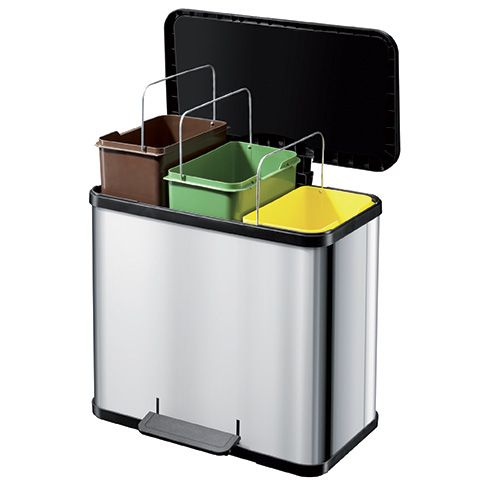
\includegraphics[scale = 0.34]{HouseholdRecyclingBin.jpg}
\caption{Household separation recycling bin}
\label{fig: Household separation recycling bin}
\end{center}
\end{figure}

There are also existing grey water systems available for purchase online or in-store. However, the setup of these systems and the size of its components usually vary case-to-case dependent on the appliances to be linked to the system, the size of the storage tank required by the household and the quality of the filtration component to be installed. Components of a grey water system can be easily purchased by any individual, but some degree of expertise and knowledge in the field is usually required to correctly size components, determine how they will function together and physically setup the system with the household's present water supply system. 

The design for \ac{e-casa}'s expected to be much like the one in Figure~\ref{fig: Grey water system} as it will be linked to the household's shower/bath, basins, washing machine, outdoor tap and toilet.
%
\begin{figure}[h!]
\begin{center}
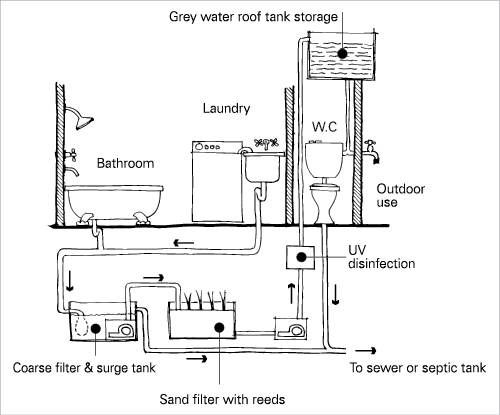
\includegraphics[scale = 1.2]{Household_Grey_Water.png}
\caption{Household grey water system}
\label{fig: Grey water system}
\end{center}
\end{figure}
%
A number of different household composters are available on the South African market. These composters are easily accessible and available online and in hardware stores. It is assumed for the time being that a 220 \textit{litre} composter (shown in Figure~\ref{fig: Outdoor Composter}) will be of sufficient size to store a household's organic and garden refuse waste.
%
\begin{figure}[h!]
\begin{center}
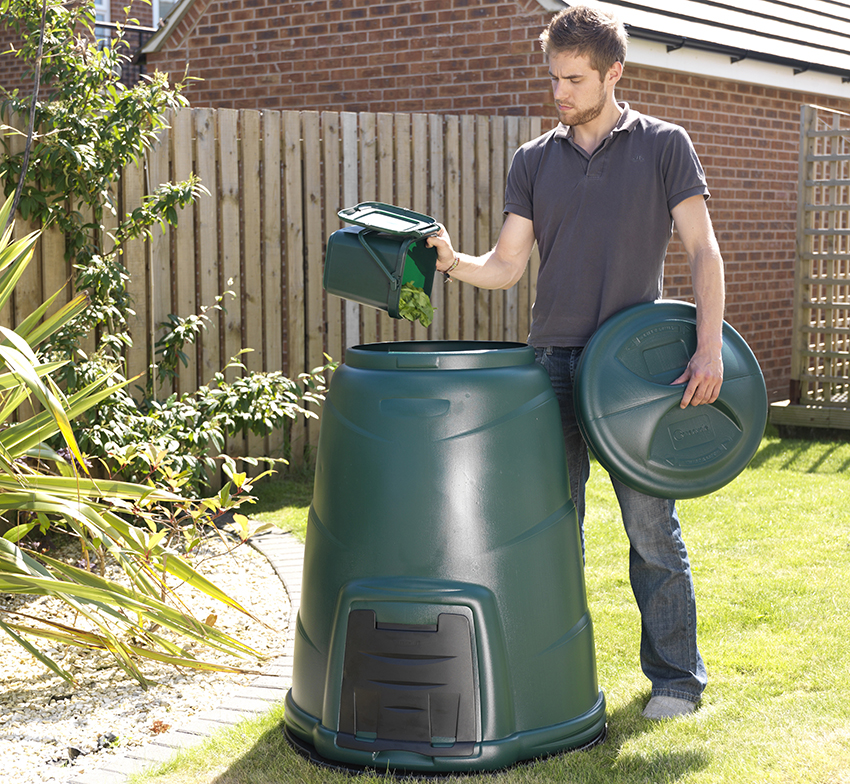
\includegraphics[scale = 1.1]{Outdoor_Composter.jpg}
\caption{Outdoor Household Composter (220 \textit{litres})}
\label{fig: Outdoor Composter}
\end{center}
\end{figure}

\subsection{Need Validation}
\textcolor{red}{Need to review: Present scenarios and evaluate what the metrics would do.}\\

To ensure the proposed system can fufill the identified need, metrics have been developed that will be used to evaluate the performance of the system.
%
\begin{table}[h!]
\caption {System Performance Metrics} \label{tb: Performance_Metrics} 
\begin{center}
\begin{tabular}{p{5cm}|p{3cm}|p{8cm}}\toprule
	{\textbf{Metric Category}} & {\textbf{Unit Measure}} & {\textbf{Description}}\\ \midrule
    Water savings & \textit{litres} & The volume of water saved is calculated as the reduction in the volume of water that enters the household. This value is already measured by the household's municipality that bills them for water usage each month.\\
    \hline
    *Organic waste reduction & \textit{kilogram} & The total mass of organic waste re-used by means of composting is the reduction in household waste output.\\
    \hline
    Disposable waste reduction & \textit{kilogram} & The total mass of plastic, paper and glass respectively represent disposal waste reduction. It is assumed firstly, that all disposable materials would not have been recycled before system implementation and secondly, that all disposable materials will ultimately be recycled by the municipality's garbage management system.\\
    \hline
    Household service cost saving & \textit{Rands} & The reduced water consumption of the household and the re-used organic waste helps to perform household activities that would otherwise require a homeowner to purchase more water, compost and vegetables. This includes the municipal water used in the household and compost for a vegetable garden. Household service cost saving is thus the total monetary savings obtained from reduced water use, self-composting and not having to purchase vegetables as frequently.\\
    \hline
    Payback Period & \textit{years} & The payback period is defined as the period of time it takes for the financial savings generated by the system, to equal the initial cost of purchasing and installing the \ac{e-casa} system. \\ \bottomrule
\end{tabular}
\end{center}
\end{table}
%
*= Problem to measure

The five metrics in Table~\ref{tb: Performance_Metrics} are to be evaluated using different hypothetical scenarios. These scenarios reflect expected environmental conditions and consideration of the metrics in conjunction with these scenarios is used to determine the appropriateness of the system. The hypothetical scanarios are as follows:
%
\begin{description}
	\item[Municipal water restrictions] - If the local municipality decided to place water restrictions in the area of the household and the household's water use was currently above that threshold, the water savings metric would be used to determine whether the household could reduce their water consumption enough by installing the system to fall under the specified limit.
	\item[Equipment price rise] - If the price of grey water system equipment rises substantially due to unfavourable economic circumstances or exchange rate changes before the \ac{e-casa} system is installed, the payback period will significantly increase as more capital would have to be earned back in the form of savings which would take a longer period of time.
\end{description}

The metrics are shown to be helpful in assessing the performance of the system under differential external operating conditions (the hypothetical scenarios given above). 
%As defined by the metrics, the system is believed to achieve the objectives laid out by the defined need. Thus the system is able to fufill the identified needs.

\section{Concept Exploration}
\subsection{Operational Requirements Analysis}
\textcolor{red}{analysing the stated operational requirements in terms of their objectives. Restating, redefining or amplifying (as required) to provide specificity, independence and consistency among different objectives}

\subsection{Performance Requirements Formulation}
\textcolor{red}{Translating operational requirements into subsystem functions and defining a necessary and sufficient set of performance characteristics reflecting the functions essential to meeting the system’s operational requirements. Formulating the performance parameters required to meet the stated operational requirements.}

Subsystem functions are allocated and represented by the following \ac{FBD}s:\\ \textcolor{red}{NOTE TO SELF: Add labels to one of the FBDs}
%
\begin{figure}[h!]
\begin{center}
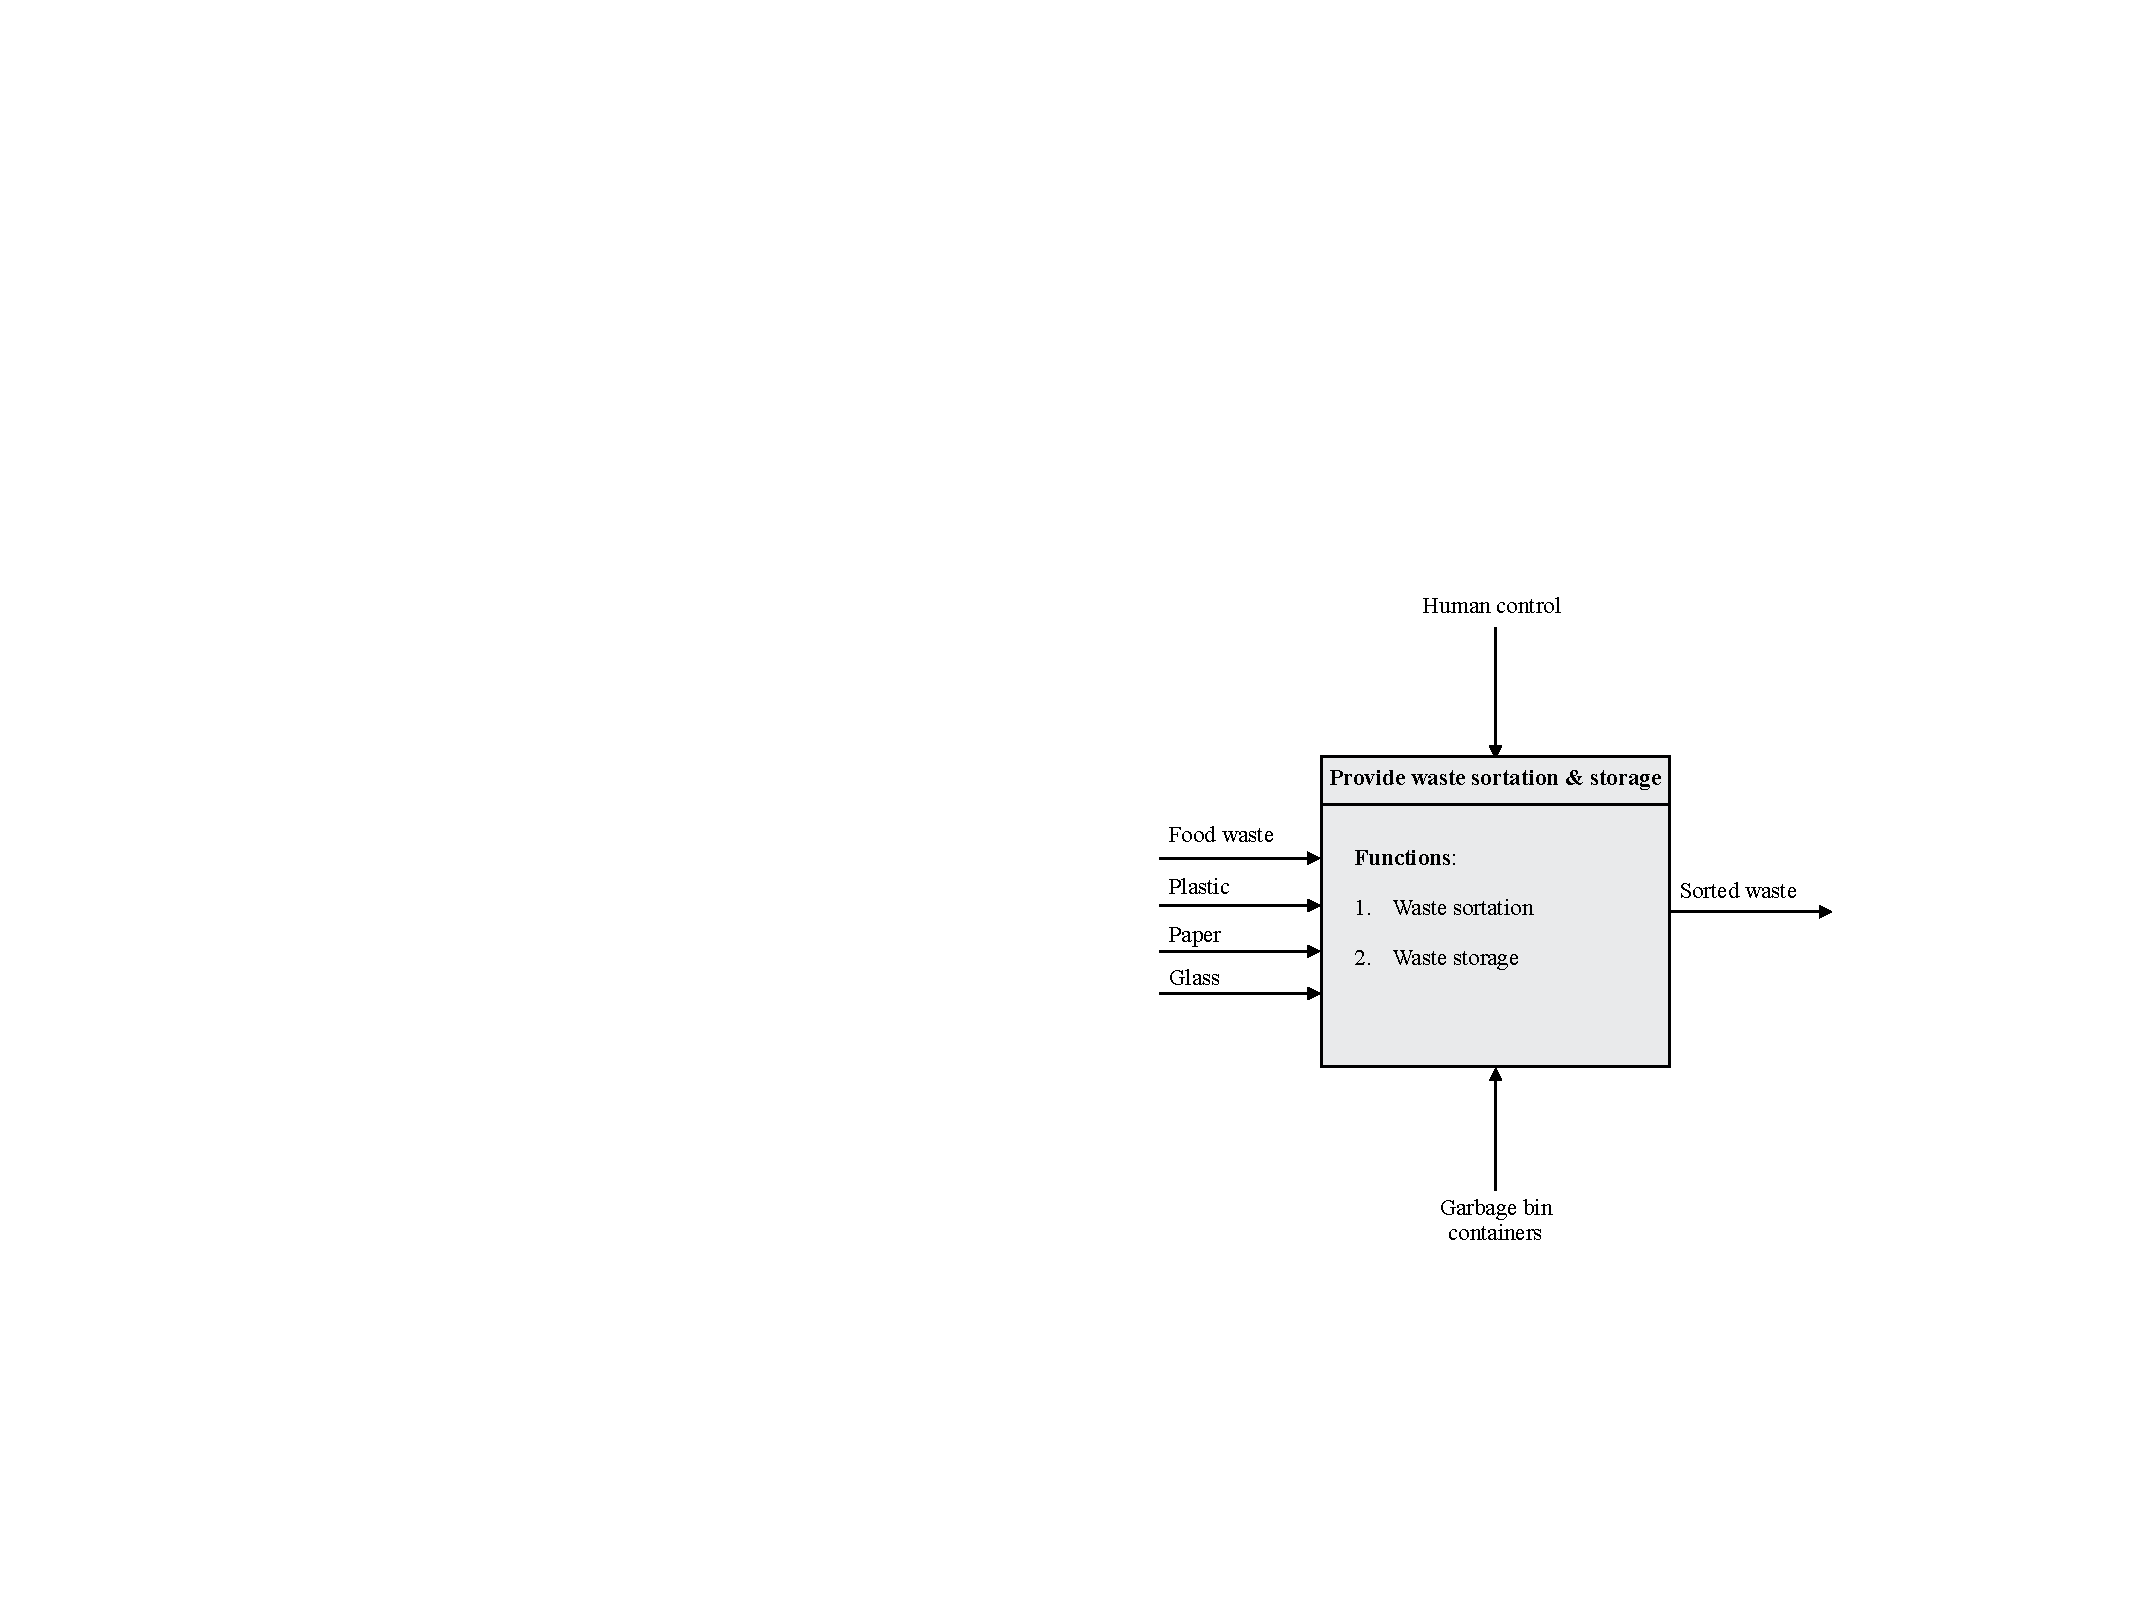
\includegraphics[scale = 0.8]{Function1.pdf}
\caption{Provide waste sortation and storage}
\label{fig: Function1}
\end{center}
\end{figure}
%
\begin{figure}[h!]
\begin{center}
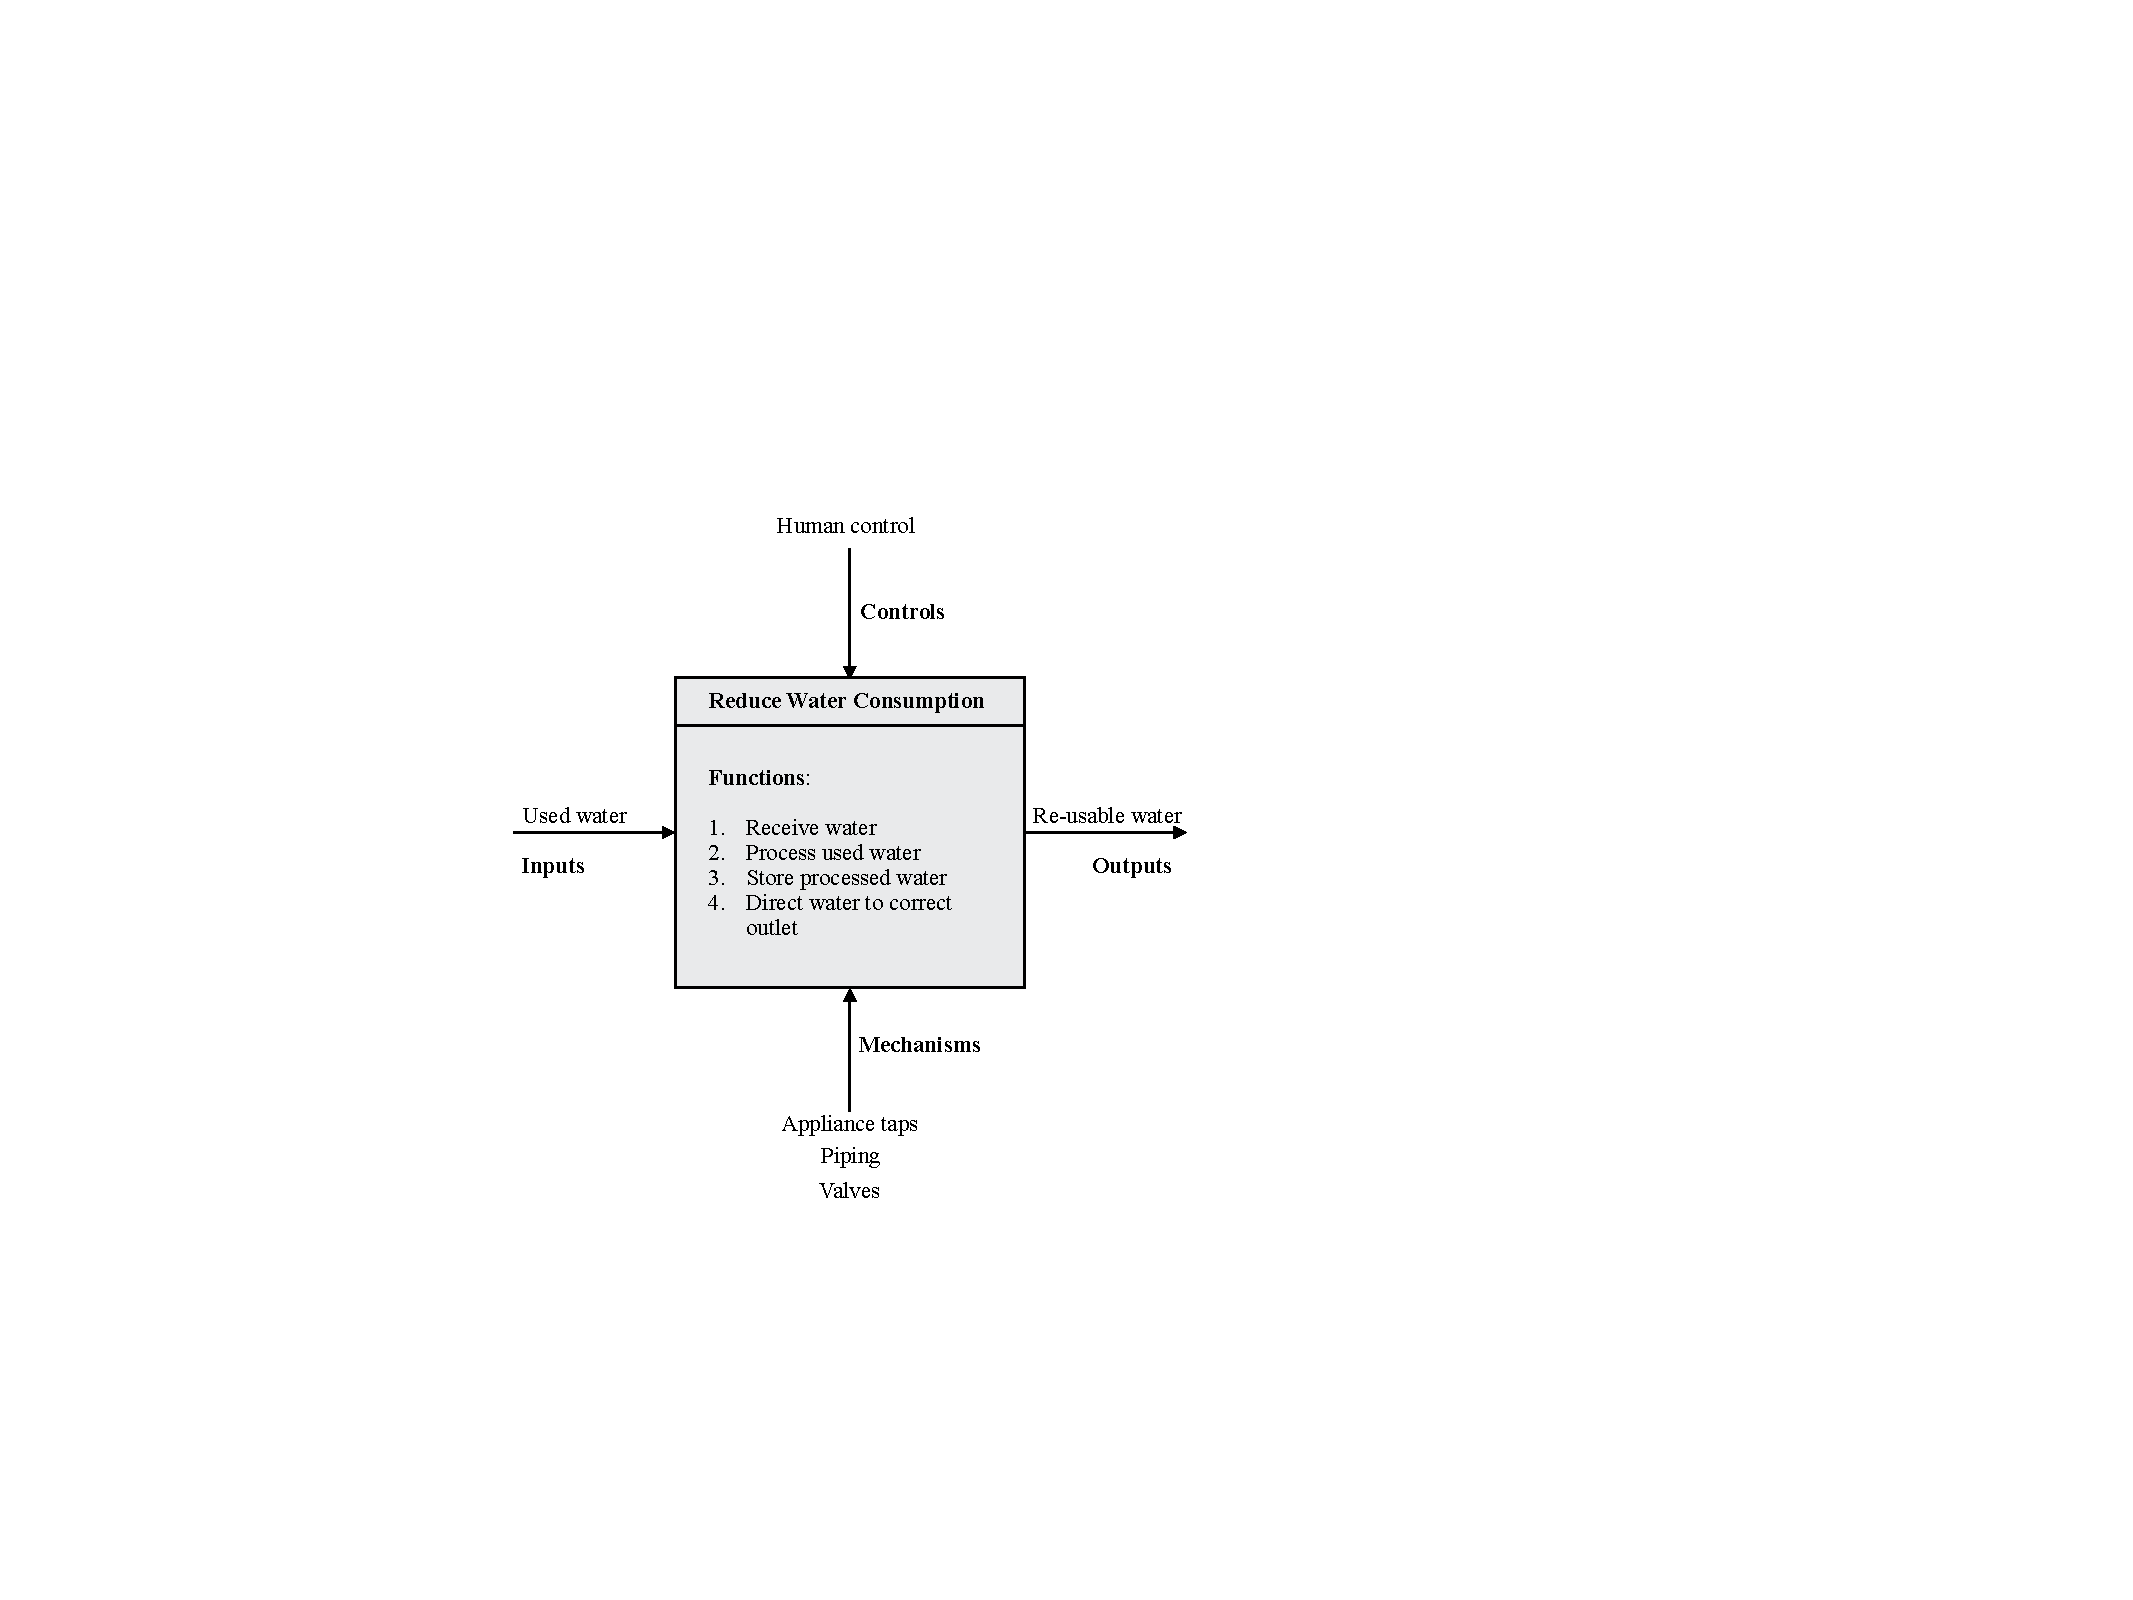
\includegraphics[scale = 0.8]{Function2.pdf}
\caption{Reduce water consumption}
\label{fig: Function2}
\end{center}
\end{figure}
%
\begin{figure}[h!]
\begin{center}
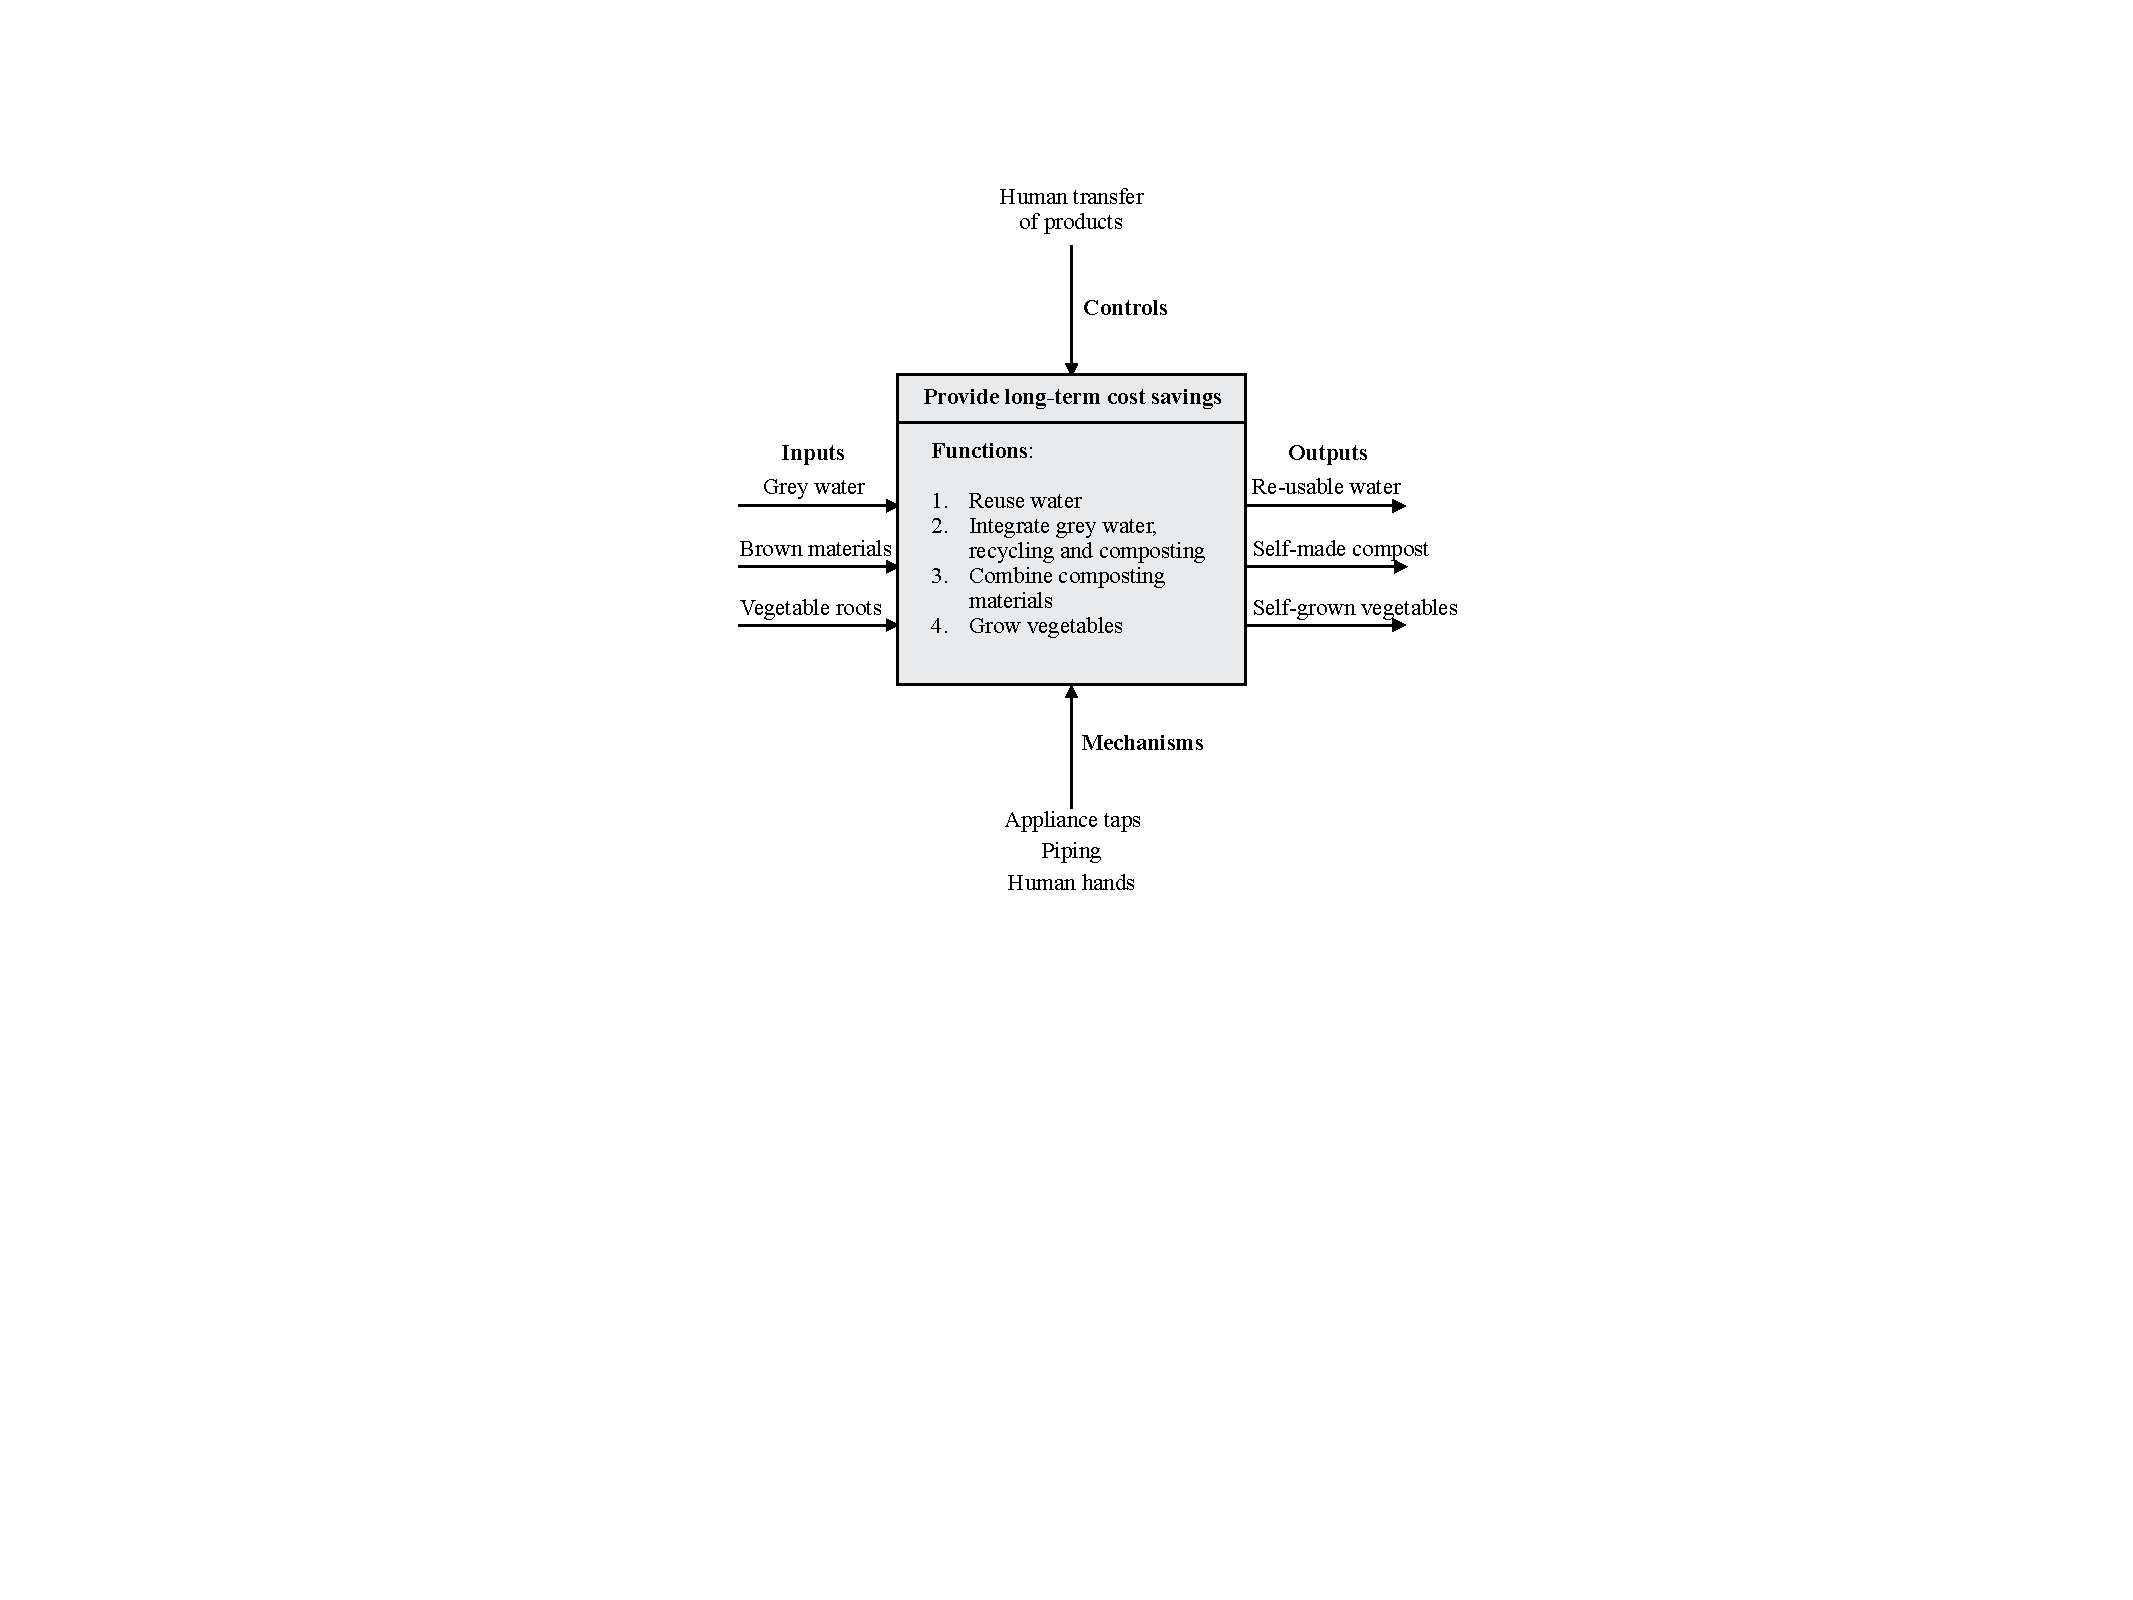
\includegraphics[scale = 0.8]{Function3.pdf}
\caption{Provide long-term cost savings function}
\label{fig: Function3}
\end{center}
\end{figure}

\subsection{Implementation of Concept Exploration}
\textcolor{red}{Exploring a range of feasible implementation technologies and concepts offering a variety of potentially advantageous options.}

Multiple alternatives for each of the function tasks given in \ac{FBD}s are explored in Table~\ref{tb: FunctionalTasks}.
%
\begin{table}[h!]
\caption {System Alternatives for Functional Tasks} \label{tb: FunctionalTasks} 
\begin{center}
\begin{tabular}{p{3.5cm}|p{6cm}|p{6cm}}\toprule
	{\textbf{Functional Task}} & {\textbf{Alternative 1}} & {\textbf{Alternative 2}}\\ \midrule
    Waste sortation and storage & One garbage bin with multiple compartments & Multiple garbage bins each with a single compartment\\
    \hline
    Receive water & Four separate pipes from (bath, shower, basin and washing machine) that connect to the central grey water storage tank & One pipe that merges bathroom appliance outputs and one for the kitchen. These two pipes will feed water to the central grey water tank\\
    \hline
    Process used water & Filter grey water to be sent back to the washing machine for re-use and to the garden (for composting and plant watering) and toilet cistern (for flushing) & Do not purchase a filter and only use grey water in the garden and to flush the toilet cistern\\
    \hline
    Store processed water & Large central tank to store all water received until it is needed again by the washing machine, toilet cistern or in the garden & Smaller central tank to store used water only for use in the garden\\
    \hline
    Direct water & Five-way water valve to direct grey water back to the washing machine, to an outside water tap (to be used in a compost container), to the garden's sprinkler system (to water the vegetable patch) and to the toilet cistern & Three-way valve to direct grey water back to outside water tap to be used in a compost heap and to the garden's sprinkler system to water the vegetable patch\\
    \hline
    Re-use water & Grey water system makes water available for re-use at necessary outlet points when human user demands it at a tap & Grey water system makes water available for re-use at necessary outlet points in the required quantities (specifically at the garden's sprinkler system to eliminate the need for the user to retrieve the water and use it themselves)\\
    \hline
    Integrate water, recycling and composting & N/A - Alternatives explored by other system functions & N/A - Alternatives explored by other system functions\\
    \hline
     Combine composting materials & Purchase a residential size compost container that the necessary materials are combined in to produce compost & Create a large compost heap in the household's garden to store and mix compost materials. Construct a structure to shelter this compost and fix it in place\\
    \hline
     Grow vegetables & User must collect water from the outside garden tap in the necessary quantity and use it to water the vegetable patch. Compost collected and filled in the vegetable patch manually by human user & Connect grey water storage tank directly to garden sprinkler system to be activated by the human user at the flick of the sprinkler switch. Compost collected and filled in the vegetable patch manually by human user\\
    \hline
    \bottomrule
\end{tabular}
\end{center}
\end{table}
%
	
\subsection{Performance Requirements Validation}
\textcolor{red}{Conducting effectiveness analyses to define a set of performance requirements that accommodate the full range of desirable system concepts and validating the conformity of these requirements with the stated operational objectives and refining the requirements if necessary.}

\section{Concept Definition}
\subsection{Performance Requirement Analysis}
\textbf{System performance requirements refinement} - The system performance requirements do not consider the impact the size of the household may have on them and are these performance requirements are rather set using data for an “average” household in South Africa. The size of the household will affect the size of the required system, the cost of such a system and therefore the system’s ability to be financially feasible. The waste producing capacity of a smaller household is a constraining requirement as smaller households will produce less waste and it will take longer to realise the cost savings of a larger system (possibly more than 2 years). However, smaller households will require smaller system components and therefore a lower initial system cost than a larger system.

To ensure the long-term operation of the system, each subsystem must be made easy for the system user him/herself or cheap labour to maintain. Standardised components are therefore preferred for the greywater system as well as the physical waste system. 

\textbf{Updated performance requirements}
The following performance requirements were included in the specification following the after reviewing the initial performance requirements.

\subsubsection{Relating analysed spesifications to operation needs}

\subsection{Functional Analysis and Formulation} 
\textcolor{red}{Allocating subsystem functions to the component level in terms of system functional elements and defining element interactions, developing functional architectural products, and formulating preliminary functional requirements corresponding to the assigned functions.}
%
\begin{table}[h!]
\caption {Functional subsystem elements} \label{tb: Functional_SS_elements} 
\begin{center}
\begin{tabular}{p{4cm}|p{4cm}|p{4cm}|p{4cm}}\toprule
	{\textbf{Subsystem}} & {\textbf{Class function} & {\textbf{Element Function}} & {\textbf{Physical Elements}}\\ \midrule
    \textcolor{Format used by sample project} & ... & ...\\
    \hline
    ... & ... & ...\\

    \bottomrule
\end{tabular}
\end{center}
\end{table}
%
\subsection{Concept Selection}
\textcolor{red}{Synthesizing alternative technological approaches and component configurations designed to performance requirements; developing physical architectural products; and conducting trade-off studies among performance, risk, cost, and schedule to select the preferred system concept, defined in terms of components and architectures.}

The alternatives given for the functions in Table~\ref{tb: FunctionalTasks} were assessed according to financial feasibility, convenience and ease of implementation. One alternative was selected for each function (Table~\ref{tb: chosen_Alts}) with the explanation for choice in each alternative given below:

\textbf{Recycling and waste disposal tasks}\\
For waste sortation, alternative one will be selected in order to save space and keep the garbage bin as small as possible to fit into the household's kitchen.\\

\textbf{Grey water tasks}\\
To receive water, the alternative with the least invasive way of changing the household's current piping system will be selected (which is anticipated to be ?). With regards to the processing of used water, alternative two will be selected. This is because the filter is a significant expense and will require frequent maintenance. The significant expense and inconvenience of alternative one is anticipated to outweigh its financial benefit as this would only save water being demanded by the household's washing machine.\\

Alternative two for used water storage goes hand-in-hand with alternative two for water processing. Because a filter will not be purchased for the grey water system, a smaller central tank will be used to temporarily store used water until it is demanded for vegetable garden and composting activities. Alternative one is chosen for the re-use water function. Water will be made available for re-use by the grey water system that will make it available at the outside garden tap and sprinkler system for the user. It is then up to the user to use (re-use) this water as best possible.

Alternative two would provide more value to the system user but would require substantial, research, financial investment and testing to develop and automated system that caters specifically to the household's unique needs. For the direct water function, alternative two will be selected as only a two-way valve will be needed if water is not to be re-directed from the storage tank to the washing machine for use.\\

\textbf{Financial savings related tasks}\\
The function of integrating water, composting and recycling will be performed both by hardware and the human user. Hardware (piping) will be used to connect the grey water subsystem directly to the outside sprinkler system surrounding the vegetable patch and to an outside tap for garden water usage. Grey water directed to the outside tap will need to be collected in the necessary quantity by the human user and input into the compost container. The human user will also be required to create the link between the recycling system and the compost system by means of physically transporting paper waste, garden refuse and food clippings to the compost container. There is no alternative for this option because alternatives for integrating these subsystems in different ways are explored through the other function tasks.

Alternative one will be selected to combine composting materials. Although a large garden compost heap may produce more compost than a smaller compost container, the smaller residential compost container is more convenient for the human user. To maintain a large compost heap in the garden (alternative two) is not practical for all households due to: space restrictions, the need for a structure to protect the compost from weather conditions that will change the balance of water in the heap and the cost of such a structure. The function of combining the composting materials will be performed by the human user who will place the required amounts of dry materials, food waste, paper and brown materials into the residential size compost container.

The task of growing vegetables will need to be performed by the human user. However, fulfilling this function will be made easier for the human user by selecting alternative two that will connect the household's water sprinkler system directly to the grey water storage tank. This way the user will just have to flick a switch to turn on the sprinklers and water the vegetable garden instead of manually collecting water from a tap and watering the growing vegetables. Although alternative two is expected to be more expensive because of the hardware required, it is expected to add a significant benefit to the system user in the form of convenience. The compost to grow vegetables will have to be collected out of the bottom of the compost container by the human user and placed into the vegetable patch. This is because there is not yet a way to automate this process feasibly on such a small scale.

The system as whole must be as cost effective as possible. However, quality should not be sacrificed for unreliable components. The grey water system components will be selected with the intention of a minimum 50 year project life for each, as per industry piping standards. \citep{Fischer2012}. This is important to ensure the system does not require large-scale repairs over the life of the project, only routine maintenance and reparis. The labour and expertise required to make system repairs for the installed grey water system are expected to be costly and should be avoided.
%
\begin{table}[h!]
\caption {Functions and their selected alternatives} \label{tb: chosen_Alts} 
\begin{center}
\begin{tabular}{p{3.5cm}|p{9cm}}\toprule
	{\textbf{Function/Task}} & {\textbf{Selected Alternative}\\ \midrule
    Waste sortation and storage & One garbage bin with multiple compartments \\
     \hline
     Receive water & Four separate pipes from (bath, shower, basin and washing machine) that connect to the central grey water storage tank \textcolor{blue}{One pipe that merges bathroom appliance outputs and one for the kitchen. These two pipes will feed water to the central grey water tank}\\
    \hline
    Process used water & Filter grey water to be sent back to the washing machine for re-use and to the garden (for composting and plant watering) and toilet cistern (for flushing) \textcolor{blue}{Do not purchase a filter and only use grey water in the garden and to flush the toilet cistern}\\
    \hline
    Store processed water & Large central tank to store all water received until it is needed again by the washing machine, toilet cistern or in the garden \textcolor{blue}{Smaller central tank to store used water only for use in the garden}\\
    \hline
    Direct water & Five-way water valve to direct grey water back to the washing machine, to an outside water tap (to be used in a compost container), to the garden's sprinkler system (to water the vegetable patch) and to the toilet cistern \textcolor{blue}{Three-way valve to direct grey water back to outside water tap to be used in a compost heap and to the garden's sprinkler system to water the vegetable patch}\\
    \hline
    Re-use water & Grey water system makes water available for re-use at necessary outlet points when human user demands it at a tap\\
    \hline
    Integrate water, recycling and composting & N/A - Alternatives explored by other system functions\\
    \hline
     Combine composting materials & Purchase a residential size compost container that the necessary materials are combined in to produce compost\\
    \hline
     Grow vegetables & User must collect water from the outside garden tap in the necessary quantity and use it to water the vegetable patch. Compost collected and filled in the vegetable patch manually by human user \textcolor{blue}{Connect grey water storage tank directly to garden sprinkler system to be activated by the human user at the flick of the sprinkler switch. Compost collected and filled in the vegetable patch manually by human user}\\
    \hline
    \bottomrule
\end{tabular}
\end{center}
\end{table}
%
The selected alternative for each function will be chosen to form the final system.

\subsection{Concept Validation}
\textcolor{red}{Conducting system analyses and simulations to confirm that the selected concept meets requirements and is superior to its competitors and refining the concept as may be necessary.}

\chapter{Engineering Development Phase}
\textcolor{red}{analysing the system functional specifications with regard to their derivation from operational and performance requirements and the validity of their translation into subsystem functional requirement identifying components requiring development}

The system's functional specifications are translated into three subsystem functional requirements:\\

\textbf{Grey Water subsystem} - This system interfaces with the household's municipal water supply which is its primary input. It is also connected to multiple household components, namely: the washing machine, bath/shower, toilet cistern and garden. This subsystem has three functional capabilities. The first being to store grey water in a central tank to be recycled (re-used) in the system, secondly to sort re-usable water from unusable waste water and finally to transfer both the re-usable and unusable water in the subsystem to the appropriate destination (component). This subsystem also feeds grey water to the next subsystem (compost).\\

\textbf{Compost subsystem} -  The compost subsystem interfaces with the household's garden and organic material stockpile components. It uses organic materials from the material stockpile to provide compost to the garden component. It's primary capabilities are to store organic materials and provide some form of visual management for the user to know when there is sufficient compost for the storage container to be emptied. This subsystem is connected to the grey-water subsystem which provides grey water as an input as well as to the Recycling and waste disposal subsystem which provides paper and other organic waste to the compost system.\\

\textbf{Recycling and waste disposal subsystem} - This subsystem interfaces with the household's kitchen as a component in order to receive all household waste as an input. It also intrefaces with the municipal recycling system at the point where waste is placed on the sidewalk for collection by the municipality's waste collection service. Its primary capability is to sort household waste into the relevant categories for re-use or disposal. Paper recyclables and organic waste collected by this subsystem are output to be used in the compost subsystem while other recyclables and non-recylable waste is disposed of to the municipal recycling system.
%
\begin{figure}[h!]
\begin{center}
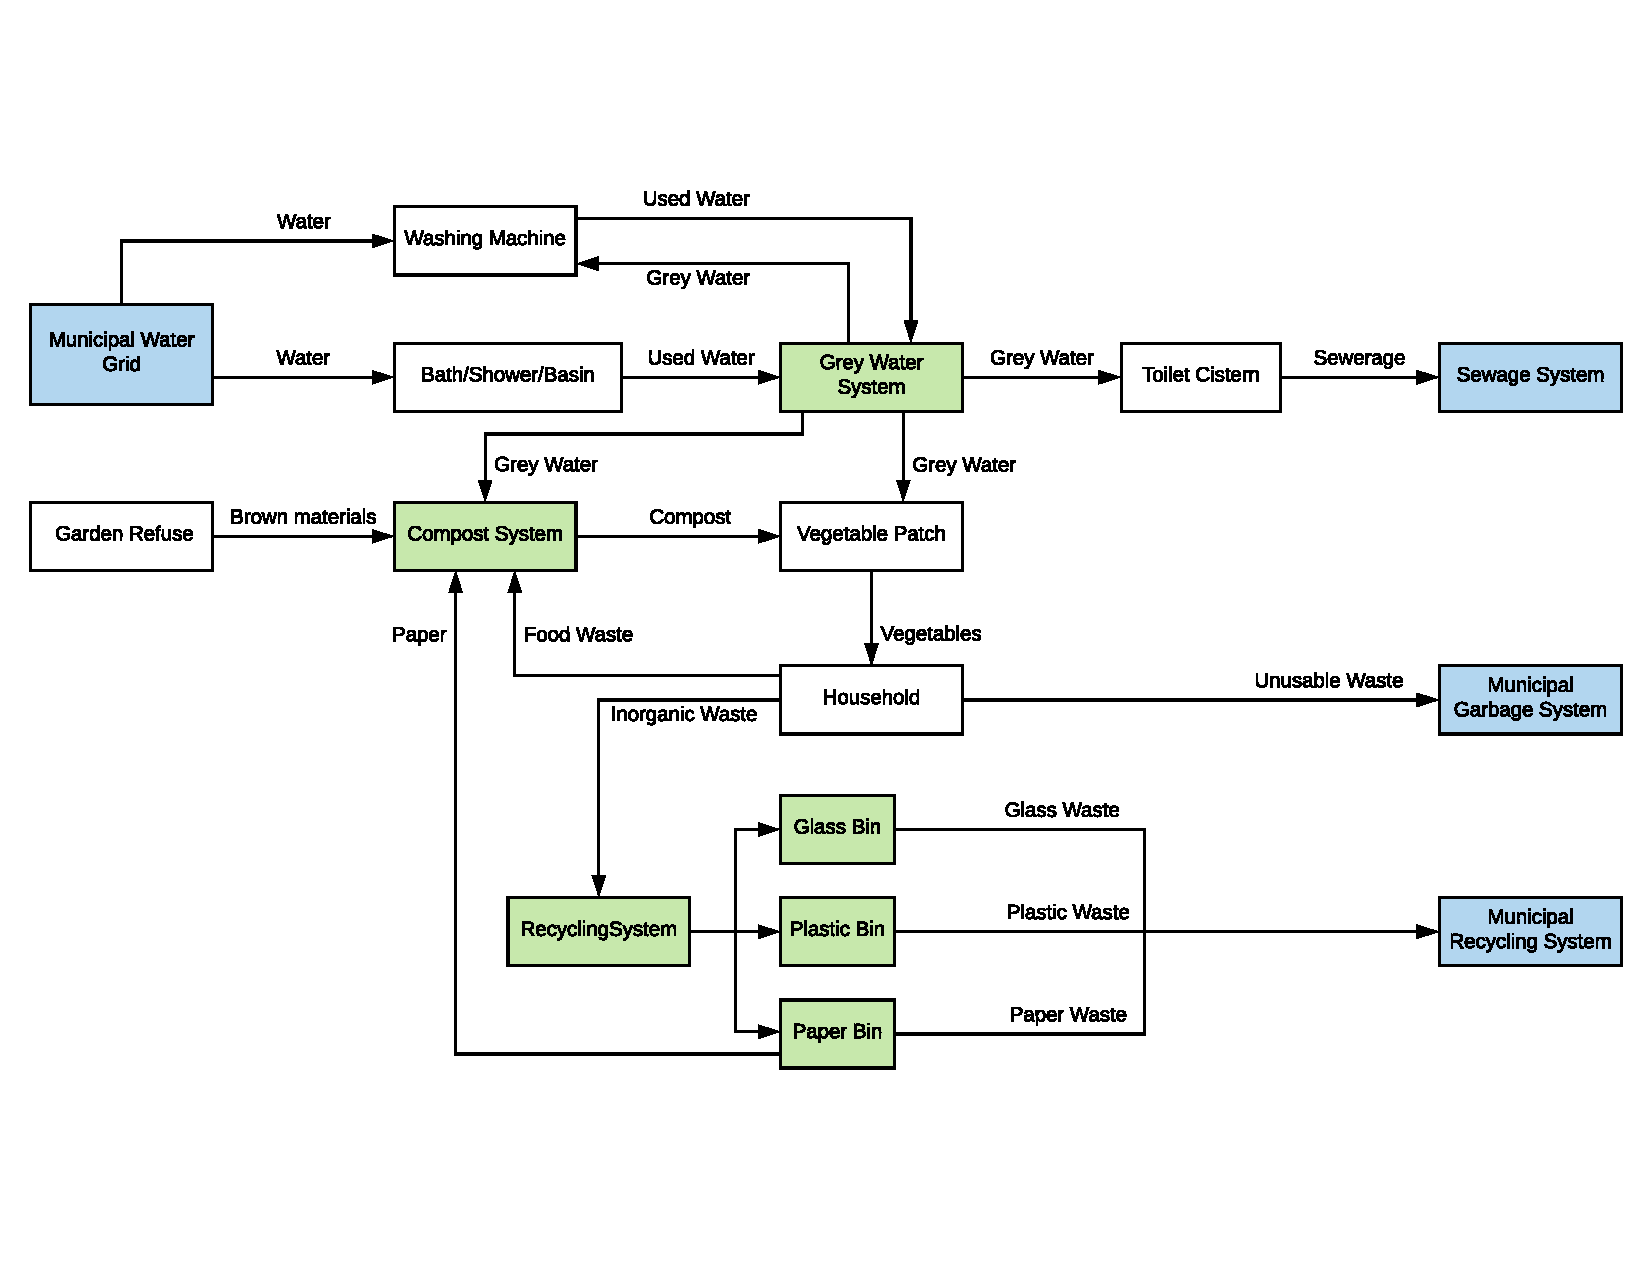
\includegraphics[scale = 0.55]{System_Diagram.pdf}
\caption{System Diagram}
\label{fig: systemDiagram}
\end{center}
\end{figure}
%
\section{Advanced Development Phase}
The components for the three aforementioned subsystems of \ac{e-casa} have already been designed and can be purchased from the market. The components will therefore not be evaluated individually but \ac{e-casa} is unique in that it is the first system of this kind that integrates these different components .
For this reason, the advanced development phase for the selected concept will be conducted to identify possible implementation risks of using these components together as one system.

\subsection{Requirements Analysis}

\subsection{Functional Analysis and Design}

\subsection{Prototype Development}
%
\begin{table}[h!]
\caption {Selected alternatives and their associated risks} \label{tb: Functional_SS_elements} 
\begin{center}
\begin{tabular}{p{7cm}|p{7cm}}\toprule
	{\textbf{Selected Alternative}} & {\textbf{Associated Risk}\\ \midrule
    \textcolor{Format used by sample project} & ... & ...\\
    \hline
    ... & ... & ...\\

    \bottomrule
\end{tabular}
\end{center}
\end{table}
%

\subsection{Development Testing}
%
\begin{table}[h!]
\caption {Associated risks and applicable risk mitigation plans} \label{tb: Functional_SS_elements} 
\begin{center}
\begin{tabular}{p{3cm}|p{5cm}|p{5cm}}\toprule
	{\textbf{Function} & \textbf{Associated Risk}} & {\textbf{Risk Mitigation}\\ \midrule
    \hline
    Process used water & Water processor unit (filter) malfunctions and pollutants pass through to garden and washing machine water & ?\\
     \hline
    Direct water & One path on five-way water valve is damaged and causes water to leak out & ?\\
     \hline
    Waste sortation & User places disposable waste into incorrect category (i.e. plastic into paper or paper into glass) & Use visual management signals or colours to mark gardbage bin compartments clearly
\\
    \hline
Grey water storage supply & Not enough water to irrigate vegetable patch & Provide storage tank or buffer to offset needs\\
    \bottomrule
\end{tabular}
\end{center}
\end{table}
%
%
\begin{table}[h!]
\caption {Design specification and motivation for selected alternatives} \label{tb: Functional_SS_elements} 
\begin{center}
\begin{tabular}{p{4.5cm}|p{4.5cm}|p{4.5cm}}\toprule
	{\textbf{Selected Alternative}} & {\textbf{Design Specification}} & {\textbf{Motivation}}\\ \midrule
    \hline
    Waste sortation and storage & One garbage bin with 3x removable 20~\textit{l} containers& ...\\
        \hline
    Receive water & 4x Separate pipes that connect as inputs to central grey water tank & Entire grey water system does not need to stop when one line of supply (pipe) is damaged. Damaged line can be switched off to prevent water flow while others continue to operate\\
        \hline
    Process used water & Water filter that is capable of removing enough contaminats for the water to be used in a washing machine & If the water is safe enough to be used in the washing machine, it will be safe enough to use in the garden and toilet cistern \\
        \hline
    Store processed water & ?~\textit{l} tank to store sufficient water for the three outlets: washing machine, garden and toilet cistern & Smaller tank would not enable household to earn as much financial savings and the payback period would increase for the household\\
        \hline
    ... & ... & ...\\

    \bottomrule
\end{tabular}
\end{center}
\end{table}
%
\section{Engineering Procurement Phase}
\textcolor{red}{The advanced development phase has selected specifications of the chosen alternative components in order to meet the design requirements. The engineering design phase will now deal with the reliability and maintainability of components that are producible and affordable in consideration of the interface elements. - SAMPLE GROUP'S ANSWER}

\subsection{Requirements Analysis}
\textcolor{red}{The system design requirements are analysed for consistency and completeness, this is to avoid any systems requirements that would contradict each other and are unable to meet the specified need. This is also done to verify that the system meets the specifications and operational requirements. Identifying requirements for all external and internal interactions and interfaces is done to make sure that the system would be able to interact and interface with its entities to the best level possible and be able to perform or output what is needed correctly. That is, if signals or inputs from an external entity would be transformed into the outputs that are required by the external entity. This also includes how the system should be able to adapt or perform to its environment, without giving any functional problems.
The process of systems design has a repeated circumspection back to the requirements analysis. The main design requirements of the system are that it must be easy to use, and it must be reliable. Further design requirements of importance are that the system must be producible and affordable. These design requirements are a follow up from the functional and physical requirements. - SAMPLE GROUP'S ANSWER}

\subsection{Functional Analysis and Design}
\textcolor{red}{The components of the system need to interact effectively through the available interfaces. These interfaces include physical connections through cable connections and the software that retrieves information by means of these cables and displays the result of the actions taken by the user. Integration between all the parts (i.e. the touch screen with camera, speed point machine, biometric scanner and printer) is necessary for the overall functioning of the system. Testing these interconnections may pose as a challenge since the system is needed in service throughout. Testing will then need to be done during low peak service periods. Another challenge may be posed by the multiple complex subsystems of the systems that all need to function in sync for the system objectives to be met. The user will interact with the system by means of the user interface provided through the software. The design and prototyping of the user interfaces will be based on a standard Graphic User Interface (GUI) as well as a form based interface that should help reducing the time needed to learn how to operate the system.
The components selected must be designed to meet the functional requirements. Each component’s interactions and interfaces are analysed and discussed below.- SAMPLE GROUP'S ANSWER}

%
\begin{table}[h!]
\caption {Component interactions and their interfaces} \label{tb: Components & interfaces} 
\begin{center}
\begin{tabular}{p{4cm}|p{4cm}|p{4cm}}\toprule
	{\textbf{Component}} & {\textbf{Interaction} & {\textbf{Interface}\\ \midrule
    \textcolor{Format used by sample project} & ... & ...\\
    \hline
    ... & ... & ...\\

    \bottomrule
\end{tabular}
\end{center}
\end{table}
%
\textcolor{red}{The interaction modes include the basic mode that is for regular users and is designed for speed and ease of use. Another interaction mode includes the assisted mode with an attendant to help the user to navigate the process made for physically impaired users}.

\subsection{Component Procurement}
\textcolor{red}{The next part of this system development is the preliminary design and building of prototypes, test and evaluation of user interfaces, correcting deficiencies and documenting product design. This is once again an iterative process of affirming whether the needs have been addressed through the final design and is beyond the scope of this task. Laying out of preliminary designs of all the required hardware and software components and interfaces needs to be done to make sure that the appropriate hardware and software are available to make this new system and it adheres to the stated need. It is also required to make sure that the software is able to interact accordingly with the hardware. This goes with implementing detailed hardware designs and software coding. The designs need to be as detailed as possible to ensure that the operational and functional needs are met with the help of the software coding. Building the prototype versions of the engineered component are essential to test the concepts. The prototype can then be used to see where mistakes or improvements can be made before the actual design is manufactured. - SAMPLE PROJECT's answer}

\subsection{Design Validation}
\textcolor{red}{A test and evaluation of the engineered products has been conducted and the results show that the engineered components meet the requirements with respect to functions, interfaces, reliability and producibility. Based on the analysis above, no deficiencies were realised as the specification descriptions were defined based on available technology that can perform system functions. The product design can be seen in the schematic below. User manuals will be accompanied by the manufacturers of the engineered components along with specifications from the programmers that have customised the software based on the system’s functional requirements. - SAMPLE PROJECT's answer}

\section{Integration and Evaluation Phase}

\subsection{Test Planning and Preparation}
\textcolor{red}{Looking at the system’s requirements to meet the specified need, these requirements have been analysed for consistence and completeness. The requirements do not contradict themselves at all which means the integration and interfaces of the required components are possible. As the components needed already exist, there won’t be a need for building specialised test equipment and facilities. Similar test equipment for ATM or the self-service kiosk will be used to ensure that the new system works efficiently. Test requirements that are needed include the ability of the machine to make use of 5.52kWH of electrical power daily, the photo quality needs to be met and the processing speed of the system would be tested before the prototype is built. The functional architecture needs to adhere to the specifications stated such as having an ergonomic setting of the kiosk which includes a touch screen keyboard, biometric scanner, camera, speed point and printer of which should all be in reach or ease of use to the user. The functional architecture would be integrated in a way similar, if not the exact system shown in figure 4, which are kiosks used at healthcare institutes in the States. An adjustable camera would be added for the convenience of people who would require using the system while sitting down (i.e. in wheelchairs or old age) and an assistant will be available to assist in filling in the required information}

\subsection{System Integration}

\subsection{Developmental System Testing}

\subsection{Operational Test and Evaluation}

\chapter{Post Development Stage}

\section{Production and Deployment Phase}

\subsection{Transitions from Development to Production}

\subsection{Production Operations}

\section{Operations and Support Phase}
\textcolor{red}{Installation and test (system integration site, internal and external, disruptive or non-disruptive installation, early system operational difficulties encountered or that could be encountered, operational personnel)
Logistics, Support and Maintenance schedule
System Upgrades (hard and software upgrade plans)}

\chapter{Software Design and System Dynamics}
\textcolor{red}{This phase is required to study the behaviour and structure of a system by carrying out sensitivity analysis tests. Only select critical elements or more as deemed fit from the designed system and apply to these to the modelling capability of a chosen software.
Your algorithm/software approach should be such that a change in the value of one element’s input can be quantitatively seen in other elements within the network. [Use software such as: Anylogic, Vensim, Stella, Dynamo++ etc]
Phase II is tied to your ability to demonstrate sensitivity analysis, structure and behaviour of a system resulting from a change in one or more parameters of some system elements.}

\section{Core 9 System Design Structure}
The main needs the system is intended to fulfill are best represented its three primary objectives: \textit{Provide Waste Sortation and Storage}, \textit{Reduce Water Consumption} and \textit{Provide long-term cost savings}. From these objectives, operational, functional and then performance requirements were developed in the earlier sections. The functional and performance requirements that \ac{e-casa} as a system is refined by are as follows:

\section{System Dynamics Analysis}
\textcolor{red}{==35marks==}

\section{Selected Elements for System Dynamics Analysis}
\textcolor{red}{==10/35marks==
Reason for selecting these elements in a situation where the new network for SD differs from the main designed network ==5/35marks==}

\section{Sensitivity Analysis}
\textcolor{red}{==20/35marks==
Simulation runs to demonstrate sensitivity analysis, changed system behaviour etc.}

\chapter{Conclusion}
\acresetall
  
\bibliography{References}

\appendix
\chapter{Some data as appendix}

\end{document}

%\textbf{Recycling and Waste Disposal Technologies} - The recycling and waste disposal subsystem can be expanded to include metal and electronic waste bins as well. However, garbage bins with more than three bins to separate waste are not commercialy available and this type of garbage bin would therefore have to be designed and built. It is particulalry advantageous to simply purchase any already existent multiple-container garbage bin because the costs that would need to be incurred to design a new one do not appear to outweigh the financial or intangible benefits to be gained. It is also expected that most households will not have enough physical space to house such a large bin and if a household did, it would be easy to purchase two three-container bins for use. Furthermore, metal and electronice waste is often found in significantly smaller quantities than more populous, plastic, paper and glass waste and it is difficulty to justify separate containers for these two waste categories as they will likely only be emptied a couple times a year.\\

%\textbf{Grey water system technologies}
	
	
%\textbf{Composting Options} - 

%A water re-use function must be provided to discern which water must be retained by the hosehold for use and which must be discarded into the municipal system based on the origin of the water. ie. Waste water from the toilet must be discarded into the municipal system but used water from the bathroom sink must be retained for re-use to flush the toilet or water the household vegetable patch. This function will also add value to the local municipality by reduce waste output and the volume of water that must be processed.\\

%\begin{description}
%	\item[Water savings (\textit{litres})] - The volume of water saved is calculated as the reduction in the volume of water that enters the household. 
%by the volume of water diverted into the grey-water system and represents a direct saving to the user.
%	\item[Organic waste reduction (\textit{kg})] - The total mass of organic waste re-used by means of composting is the reduction is household waste output.
%	\item[Disposable waste reduction (\textit{kg})] - The total mass of plastic, paper and glass respectively represent disposal waste reduction. It is assumed firstly, that all disposable materials were not previously recycled and that secondly, all disposable materials will be recycled by the municipality's garbage management system once the system is installed.
%	\item[Household service cost saving (\textit{Rands})] - The reduced water consumption of the household (from the municipality's system) and the re-used organic waste helps to perform household activities that would otherwise require a homeowner to purchase water, compost and vegetables. This includes the municipal water used in the household and compost for a vegetable garden. Household service cost saving is thus the total monetary savings obtained from reduced water use, self-composting and not having to purchase vegetables as frequently.
%	\item[Payback Period (\textit{years})] - The payback period is defined as the period of time it takes for the financial savings generated by the system, to equal the initial cost of purchasing and installing the \ac{e-casa} system. 
%\end{description}


%	\item[Long term system failure] - The water and waste savings will be realised within the first usage cycle, meaning once the system has re-used waste and waste, the saving immediately materialises. The return on investment is expected to be achieved before the onset of long term system failure. The likelihood of system failure can be decreased with continued maintenance of the system.
%	\item[External market competition] - No other competitors are presently offering an integrated system however, there are suppliers offering parts of the system. This implies that other suppliers can match or better the household service cost of the \ac{e-casa} system. The reduced cost of implementing e-casa shall lie in the simple integration with current household systems. Customers would not require large renovations to install the system, reducing the over cost and improving the return on investment making the system marketable.